\section{Numerical experiments}\label{sec:exp}

\subsection{Radiation with half-ring and full-ring reception}\label{sec:exp-radiation}

Table~\ref{tab:electrical-acquisitions} gives the electrical size of each experiment. For a square of width \(W\), we use the circumscribed radius \(a=W/\sqrt{2}\). The main synthetic experiment uses six lossless distributions on a \(96^2\) grid at \(400\,\mathrm{MHz}\), with wave speed \(3\times10^8\,\mathrm{m\,s^{-1}}\). The original arrays have ten unit-amplitude plane waves and twenty receivers at radius \(3.75\,\mathrm{m}\). Changing the aperture changes both the illumination and receiver angles. The numerical model is the scalar TM volume integral equation on the indicated grid throughout. Each synthetic noise radius is the realized Frobenius noise norm plus \(10^{-6}\|Y\|_F\), with the latter allowance covering the error of the finite-dimensional generating solve. Unless stated otherwise, a rigorous lower bound comes from outward rounding on the original grid. Area averaging the same six contrast maps to \(32^2\) and solving there changes the synthetic fields by 12.4--28.4\% on the half ring and 14.2--35.4\% on the full ring. These are differences at the reference maps. The bounds below use all \(9{,}216\) native cells.

\begin{table}[tbp]
\centering\small
\caption{Electrical dimensions and material ranges. The Manitoba rows give the frequency endpoints. Receivers are counted per illumination. In Manitoba each of two complementary groups has 12 transmitters and 12 receivers. In Fresnel the permitted receivers change with the source. The annular benchmark specifies dimensions in wavelengths. Chamber contrasts are nominal.}
\label{tab:electrical-acquisitions}
\setlength{\tabcolsep}{3.15pt}
\begin{tabular}{@{}lrrrrrrll@{}}
\toprule
Experiment & Grid & GHz & \(W\) (m) & \(W/\lambda\) & \(ka\) & \(2ka\) & \(s,p\) & Contrast\\
\midrule
Annular inclusion & \(24^2\) & -- & -- & 0.96 & 4.27 & 8.53 & \(12,48\) & \(0.1\)--\(12\)\\
Austria & \(32^2\) & 0.4 & 2 & 2.67 & 11.85 & 23.70 & \(20,40\) & \(0\)--\(3\)\\
Six shapes & \(96^2\) & 0.4 & 2 & 2.67 & 11.85 & 23.70 & \(10\)--\(32,20/32\) & \(0\)--\(3.63\)\\
Compact patch & \(12^2\) & 0.4 & 0.125 & 0.167 & 0.740 & 1.481 & \(10,20\) & \(0\)--\(0.879\)\\
Manitoba & \(40^2\) & 3 & 0.14 & 1.40 & 6.22 & 12.45 & \(12,12\) & \(1.30,\ 2.03+0.03\mathrm{i}\)\\
 & \(40^2\) & 6 & 0.14 & 2.80 & 12.45 & 24.90 & \(12,12\) & same\\
Fresnel & \(60^2\) & 4 & 0.20 & 2.67 & 11.86 & 23.71 & \(8/18,241\) & \(0,\ 0.45,\ 2\)\\
 & \(60^2\) & 6 & 0.20 & 4.00 & 17.78 & 35.57 & \(8/18,241\) & same\\
 & \(60^2\) & 8 & 0.20 & 5.34 & 23.71 & 47.42 & \(8/18,241\) & same\\
\bottomrule
\end{tabular}
\end{table}

A current in \(\ker S\) can radiate between receivers. Equation~\eqref{eq:radupper} controls the radiation retained in this space. On the \(96^2\) grid, \(\|R\|_2\simeq5.095\), whereas the leading numerical eigenvalue of the compression \(R_0\) is \(4.805\) for the half ring and \(0.544\) for the full ring. The half ring therefore leaves a much larger radiative direction unseen. For comparison, the dense receiver rings in the annular and Austria benchmarks give rigorous upper bounds \(7.56\times10^{-15}\) and \(3.03\times10^{-10}\) for \(\|R_0\|_2\), in their respective operator units. The important quantity is the projection of the radiative field onto the measured space, which depends on both aperture and sensor placement.

At \(u=0.5\) on the half ring, the tested real-sector weights fail to rule out the cap for any of the six 2\% readings. Adding the optical identity rules it out for all six. At 10\%, global optical weights pass on two objects and quadrant weights add Double chevron, with \(d>0.6227\) and \(r\simeq0.59405\). The full ring already rules out the same cap for all six with real-sector weights, at both 2\% and 10\%. This contrast isolates the value of the optical identity within each acquisition. The full- and half-ring pair does not isolate reception alone because the incident directions also change.

\begin{figure}[tbp]
\centering
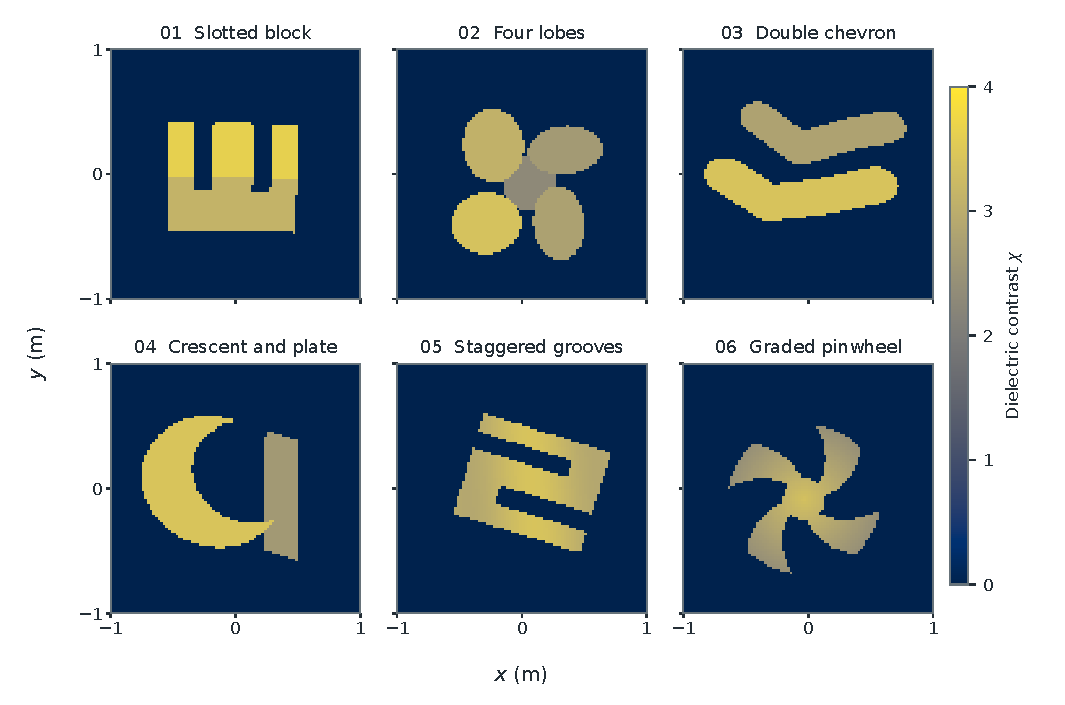
\includegraphics[width=.88\linewidth]{contrast-maps.pdf}
\caption{Reference contrasts on the \(2\,\mathrm{m}\) square, shown on a common scale. Every reported bound for these fields leaves all \(96^2\) contrast values free.}
\label{fig:contrast-maps}
\end{figure}

The reference contrasts in figure~\ref{fig:contrast-maps} have similar peaks and distinct areas and dielectric masses (table~\ref{tab:scattering-statistics}). The Born errors in this table compare the clean nonlinear field \(Y_c\) with the Born field \(Y_{\rm B}\) of the \emph{same} material on the native grid. They range from 4.07 to 6.61 relative to \(\|Y_c\|_F\). The model-wide comparison in section~\ref{sec:exp-inversion} allows the Born material to differ from the reference.

\begin{table}[tbp]
\centering\small
\caption{Native full-ring statistics. Mass is \(\int\chi\,{\rm d}A\), area includes cells with \(\chi>0\), and the Born error is \(\|Y_c-Y_{\rm B}\|_F/\|Y_c\|_F\). The right column uses the same quadrant weights on all six objects. A ratio \(d/r>1\) excludes the nonlinear material box at \(u=0.75\).}
\label{tab:scattering-statistics}
\setlength{\tabcolsep}{4.0pt}
\begin{tabular}{@{}lrrrrrr@{}}
\toprule
Object & \(\max\chi\) & Mass (\(\mathrm{m}^2\)) & Area (\(\mathrm{m}^2\)) & \(\|Y_c\|_F\) & Born error & \(d/r\), 1\%\\
\midrule
01 Slotted block & 3.632 & 2.475 & 0.739 & 4.548 & 6.614 & 2.505\\
02 Four lobes & 3.384 & 2.694 & 0.925 & 5.403 & 5.846 & 0\\
03 Double chevron & 3.416 & 2.553 & 0.811 & 5.409 & 5.715 & 0\\
04 Crescent and plate & 3.437 & 2.359 & 0.748 & 4.786 & 5.908 & 1.061\\
05 Staggered grooves & 3.408 & 2.108 & 0.671 & 4.401 & 5.996 & 1.833\\
06 Graded pinwheel & 3.346 & 1.525 & 0.550 & 5.050 & 4.069 & 0\\
\bottomrule
\end{tabular}
\end{table}

\subsection{Multiple illuminations, negative inertia and single-source bounds}\label{sec:exp-array}

At \(u=0.75\), the maximum over global weights, four-quadrant weights and two fixed sixteen-region weight fields excludes \(3,3,2,0,0\) objects at \(0.5,1,2,5,10\%\) noise, respectively (figure~\ref{fig:exclusion-envelope}(a)). The paired observations follow the original complex 2\% noise direction for each shape, with the 2\% arrays retained verbatim. A separate independent 10\% draw is used in the inversion tests below. Global weights alone pass on \(3,2,2,0,0\) objects, and the fixed sixteen-region fields pass on \(2,2,2,0,0\). The quadrant weights recover the third case, Crescent and plate, at 1\%. A uniform sector weight \(\mu_0=10^{-4}\) with optical weights \((4,16,16,16)\times10^{-6}\) gives \(d\ge0.05077102\) against \(r=0.04786783\). At 2\% this profile gives \(d/r=0.519\) for the same object. At 1\%, the best candidate from 8,987 numerical global proposals gives an upper endpoint of \(0.036671\) for that profile's lower-bound formula.

\begin{figure}[tbp]
\centering
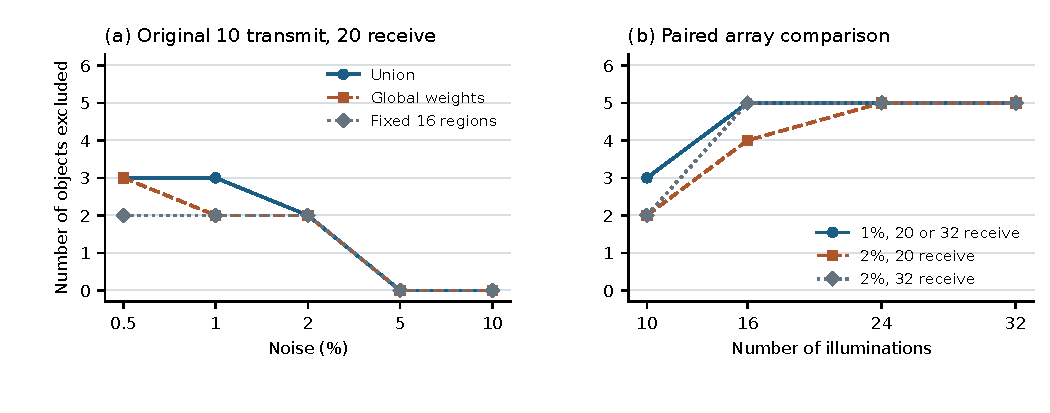
\includegraphics[width=\linewidth]{contrast-exclusions.pdf}
\caption{Excluding the full-wave cap \(u=0.75\) on six objects. (a) At the original full-ring geometry, the union over global, quadrant and fixed sixteen-region weights is nonincreasing with the paired noise level. The quadrant curve coincides with the union. (b) Increasing the number of uniformly distributed plane waves improves exclusions for both tested receiver counts. The four noise and receiver conditions shown are paired on the same materials.}
\label{fig:exclusion-envelope}
\end{figure}

For those fixed quadrant weights, \(K\) is shared by all six objects and has exactly four negative eigenvalues. The fifth eigenvalues of \(H_Y\) at 1\% in object order are \(0.010760,-0.021933,-0.022434,0.002578,0.006506,-0.022918\). Only Slotted block has a positive sixth eigenvalue as well. Four lobes and Double chevron have the largest clean norms and dielectric masses. Their positive source spectrum is exhausted by the four directions removed in Theorem~\ref{th:bound}. The decision is therefore controlled by the remaining coherent responses. For Crescent and plate, the fifth eigenvalue changes by only 4.4\% when the noise doubles, while the squared radius grows fourfold.

\begin{figure}[tbp]
\centering
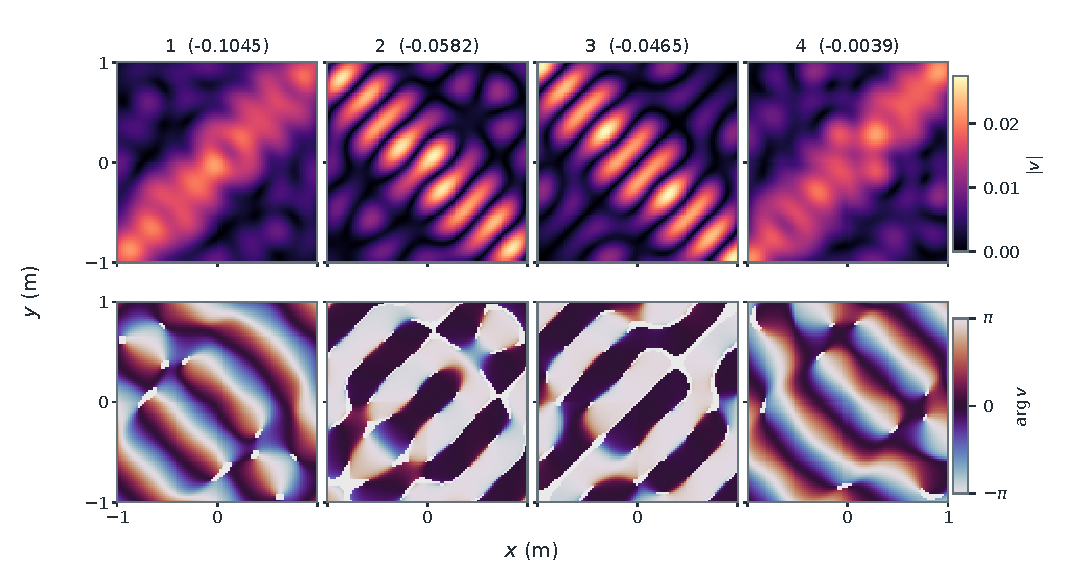
\includegraphics[width=.94\linewidth]{negative-currents.pdf}
\caption{Magnitude (top) and phase (bottom) of the four unit negative eigenvectors of \(K/\mu_0\) for the quadrant weights at \(u=0.75\). Each panel heading gives the mode index and eigenvalue. The phase is set to zero at the largest-amplitude cell and masked below 5\% of that mode's maximum.}
\label{fig:negative-currents}
\end{figure}

These four geometry-dependent directions overlap the poorly observed currents used in subspace-based inversion \cite{chen,zhong}. Each has 99.9931--99.9943\% of its energy in \(\ker S\), yet \(v^*Rv=0.01757\)--\(0.03450\) in the stored Green normalization. A 720-angle quadrature of the outgoing radiation pattern agrees with these powers to \(2\times10^{-15}\). Projection into the receiver kernel leaves almost all of this radiation. The outgoing constitutive residual \(\|(I-0.75G)v\|_2\) is at least \(1.084\) over the whole unit negative span, which is incompatible with a free mode of the uniform cap medium. Actual full-wave reference currents place only 0.23--1.60\% of their energy in this span. A rank-four, receiver-projected Fourier space generated by the nearest four corner frequencies captures 0.06--1.00\% of each mode's dark energy. With 64 Fourier columns the projection captures 99.30--99.36\%, with principal angles of \(3.2^\circ\)--\(5.9^\circ\). Figure~\ref{fig:negative-currents} thus depicts dark directions of the quadratic bound for these weights. A resonance interpretation would require a separate outgoing state test for the material of interest.

For the illumination sweep, \(s=10,16,24,32\) shots have amplitudes \(\sqrt{10/s}\), giving equal total incident fluence in the model. Receiver channels are weighted by \(\sqrt{20/p}\) for \(p=20,32\), including the same change of coordinates in the noise. On \(u=0.75\), the 1\% counts are \(3,5,5,5\) for either receiver count. At 2\%, they are \(2,4,5,5\) for \(p=20\) and \(2,5,5,5\) for \(p=32\). Graded pinwheel remains unresolved throughout. The bandwidth estimate in \eqref{eq:bandwidth} gives \(2ka=23.70\) for the full search square, and the true supports fit in circles with \(2ka=11.89\)--\(14.86\). Angular interpolation from 24 illuminations recovers independently computed clean responses at 32 illuminations with 0.0082--0.1423\% relative error. At 16 illuminations these errors are 2.63--13.42\% (figure~\ref{fig:electrical-scaling}(a)). The simulated responses change little on adding eight angles beyond 24 at the tested tolerances.

The exact negative counts of the bare reactive matrix \(I-u\operatorname{Re}_{H}G\) are \(19,21,25,36,45\) at \(u=0.75,1,1.25,1.5,2\). With fixed weights \(\mu=10^{-4}\) and \(\lambda/\mu=0.1\), the weighted counts are \(4,16,20,22,\ge39\) for 20 receivers and \(4,13,16,20,\ge34\) for 32. For these weights the \(u=2\) sums are empty even with 32 sources. At \(u=1\), 32 sources and 32 receivers at 2\% noise leave seven positive retained eigenvalues with \(d/r=0.3011\) for the strongest replayed scalar choice. At \(u=1.25\) and \(1.5\) those ratios are 0.1133 and 0.01494. Thus \(s>\nu\) can leave too little surviving source response to reach the data threshold. On the smaller annular benchmark, the fixed real-sector choice at \(u=5\) has \(\nu=4\) for 12 shots and gives \(d>0.01469\) with \(r\simeq0.010517\). The experiments resolve a competition between electrical-area growth of reactive directions and the angular bandwidth of the response. The observed thresholds belong to the tested weights and acquisitions.

\begin{figure}[tbp]
\centering
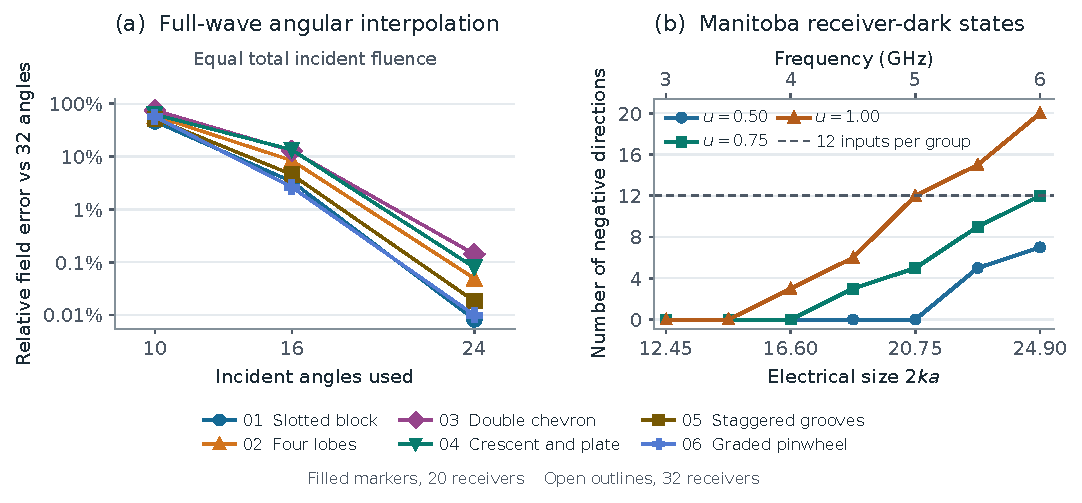
\includegraphics[width=\linewidth]{electrical-scaling.pdf}
\caption{(a) Relative error of interpolated full-wave complex responses against a 32-angle calculation, at equal total incident fluence. The points are paired by material and receiver count. (b) Numerical negative counts of the real-sector state form restricted to the receiver kernel of one Manitoba group. The dashed line marks the 12 incident fields in that group. The full state count also depends on the positive receiver term and is reported in the text.}
\label{fig:electrical-scaling}
\end{figure}

At 2\% noise, Slotted block and Staggered grooves also give a strict comparison with one coherent illumination. The joint constant-weight bounds are \(0.16069878\) and \(0.11060787\), above the respective radii \(0.09096764\) and \(0.08802506\). Theorem~\ref{th:two} gives global single-source exact fits for all unit coherent inputs. In the four-region single-source semidefinite program, receiver-exact first and second moments satisfy the local sector and optical balances and attain zero residual for every such input. Their uniform current energies are below 8,500 and 7,000 in the unweighted native coordinates. A single physical current at the stated cap has energy above 8,886.62, so these moments survive every scalar cap valid for the whole box and every coherent input. They also survive the individual error-ball energy caps \(4.983\times10^6\) and \(1.035\times10^6\). With sixteen regions the best coherent bounds are approximately \(0.18967408\) and \(0.12452151\), excluding both caps. Each resulting positive-definite state matrix leaves only one positive source eigenvalue, making the joint and best coherent values equal for that profile.

\subsection{Microwave chambers and conditional error margins}\label{sec:exp-chambers}

The Manitoba data contain four dielectric objects at seven frequencies from 3 to 6 GHz \cite{manitoba}. Two disjoint parity groups preserve \(288\) of \(552\) directed channels. Calibration uses an empty-chamber reading and a metal cylinder, with a second empty reading and a second cylinder as checks. For the four possible reference combinations, a proved distance at the primary calibration loses at most the largest field displacement to another combination. Subtracting this displacement leaves a positive passive-sector margin on \(20,5,3,1\) of the \(28\) views at caps \(0.25,0.50,0.75,1\), respectively (figure~\ref{fig:cal-headroom}). The E-shaped polyethylene object at 3.5 GHz leaves 1.358\% of the primary norm at cap 0.5, and the large nylon cylinder at 3 GHz leaves 4.018\% at cap 1. If \(\chi=x+\mathrm{i}y\) with \(x>0\), the passive-sector cap concerns \(x+y^2/x\).

\begin{figure}[tbp]
\centering
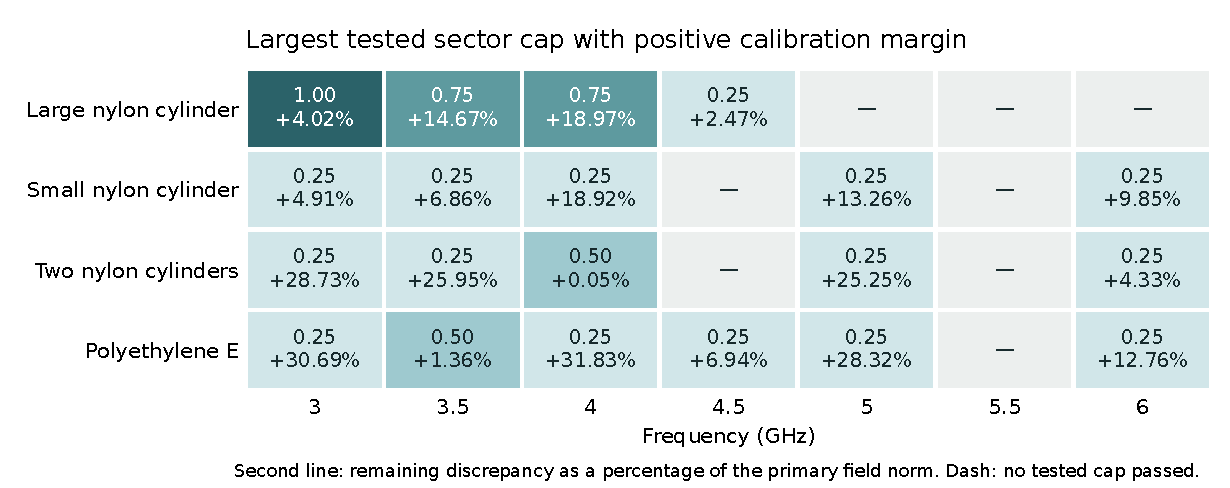
\includegraphics[width=.94\linewidth]{chamber-headroom.pdf}
\caption{Largest tested passive-sector cap with positive remaining distance after allowing any field in the convex hull of four Manitoba calibrations. The second line gives the remaining target-dependent allowance as a percentage of the primary field norm. Each row follows the same object across frequency.}
\label{fig:cal-headroom}
\end{figure}

The fixed \(0.14\,\mathrm m\) square grows from \(1.40\lambda\) to \(2.80\lambda\). At \(u=1\) the real-sector rule \(\mu=\|S\|_2^2/100\) gives full-state negative counts of \(0,0,3,8,12,15,20\) across the seven frequencies in the evaluated parity group. Restricting to \(\ker S\) gives \(0,0,3,6,12,15,20\), as in figure~\ref{fig:electrical-scaling}(b). At 5 GHz and above this choice leaves no source direction in that 12-shot group. Individual conditional margins still depend on calibration and target. The polyethylene target recovers a positive margin at 6 GHz after losing it at 5.5 GHz.

For Fresnel, we use the measured total-minus-incident fields at 4, 6 and 8 GHz, the fitted empty-field incidence and 241 receiver angles per shot \cite{fresnel}. The two individual cylinder arrangements have eight illuminations and the twin arrangement has eighteen. No tested field rules out \(u=0.5\) under the held-out empty-scene scale. At 4 GHz and \(u=0.25\), the twin arrangement's real-sector bound is 28.515\% of \(\|Y\|_F\). Inserting an additive scale of 8.884\% and a gain scale of 10.41\% into \eqref{eq:budget} leaves 6.98\% for further discrepancy. Nominal full-wave calculations with 60 and 120 cells per side differ in their full port predictions by 0.79--5.73\% across the nine views. Their residuals also include target and instrument mismatch, so these grid differences do not enclose the error of the chamber model.

The fixed-port test of the unrestricted nonnegative Born model in \eqref{eq:born} uses the actual receiver masks. In Manitoba two calibration comparisons are the difference between metal references and the empty drift plus held-out metal residual. The Born lower distances are 28.16--88.30\% of the selected field norm and exceed both scales on 25 of 28 views. In Fresnel the three lower bounds at 4 GHz are 38.36--44.85\%, above the transferred empty-field RMS scale both with and without the diagnostic complex-gain allowance. None of the six higher-frequency views exceeds both scales. These comparisons are conditional on the chosen calibration budget and the real, nonnegative Born class. Loss, antenna and three-dimensional modeling can contribute to the measured discrepancy. The experiments do not bound their combined effect on unknown loaded targets.

\subsection{Use before and during inversion}\label{sec:exp-inversion}

On the main full-ring data, the nonlinear bound rules out \(u=0.5\) for all six materials at 1\%, 2\% and independent 10\% noise. Its lower distance is 6.62--13.57 times the radius at 2\%, and 1.32--2.71 times the radius at 10\%. This calculation uses the data before any iterative inversion. Separately, the fixed finite-port test in \eqref{eq:born} rules out every nonnegative first-Born image for all 96 paired strong-scattering views in the array sweep. Its lower distances are 40.23--61.56\% of \(\|Y\|_F\). It requires one geometry-dependent weight per array. For a weak full-wave ellipse and a deliberately Born-generated control, explicit Born predictions lie in the noise balls. For full-wave paired disks with peak 0.04, the fixed weight yields zero. Selecting a direction from the data gives lower distances of \(5.348r\) and \(2.748r\) at 1\% and 2\% without restricting the Born contrast amplitude. The cheap fixed readout is consequently sufficient for these strong cases and can miss a departure from Born at small contrast. The two checks address different model classes.

\begin{table}[tbp]
\centering\small
\caption{Measured wall times, separating reusable setup from one new data matrix. The timings include numerical proposals and interval checks as stated.}
\label{tab:cost}
\begin{tabular}{@{}>{\raggedright\arraybackslash}p{.28\linewidth}
                 >{\raggedright\arraybackslash}p{.39\linewidth}
                 >{\raggedright\arraybackslash}p{.23\linewidth}@{}}
\toprule
Test & Setup or cold computation & Per new reading after setup\\
\midrule
Fixed port weighting, \(96^2\) & \(0.2\)--\(0.8\,{\rm s}\) per array & about \(0.5\,{\rm ms}\)\\
Full-wave cap test, \(96^2\) & \(57.54\,{\rm s}\) for stationary responses, \(3.84\,{\rm s}\) for negative gaps & \(5.89\,{\rm ms}\) median for six profiles\\
Initial state checks, \(96^2\) & \(1.33\)--\(34.75\,{\rm s}\) per profile & --\\
Full-wave cap test, \(12^2\) & \(0.70\)--\(0.74\,{\rm s}\) cold per reading & --\\
\bottomrule
\end{tabular}
\end{table}

Among the six large scatterers, the lower bound itself rules out a fit within \(2.5r\) for 15 of the 23 excluded object--noise--cap conditions. In the eight remaining eligible conditions, zero-start, penalized full-wave fits retained residuals above \(2.5r\) after up to 94 objective calls. An ordinary residual check would already reject those reconstructions. We therefore tested the intervention on a separately designed compact patch with peak 0.879, mean 0.654 and side \(\lambda/6\). The clean field difference to the uniform \(0.5\) square sets the scale for four fixed relative noise levels of \(12.38\)--\(26.13\%\). These are repeated measurements of one constructed material. Every method sees the same physical forward map, data and radius. It starts at zero with the same spatial penalty and the same budget. The low-cap algorithm converges to the uniform \(0.5\) square in six calls, achieving residuals of \(1.487\)--\(2.481r\), within a lenient \(2.5r\) stopping threshold. The full-box lower bound is \(1.437\)--\(2.422r\), so all configurations below that cap miss the stipulated noise ball.

Broad release to cap 2 gives residuals of \(0.991\)--\(0.992r\) and reduces separately simulated held-out complex field error from 27.50\% to 1.32--2.52\%. The relative material error rises from 0.462 to \(0.721\)--\(0.943\), and the peak rises to 1.85--2.00. At the same six-call checkpoint as the low-cap run, the released path has relative material error \(0.315\)--\(0.317\), but only one reading falls inside \(r\). A rule using the exact point discrepancy releases the cap for all four views and reaches nearly the same final errors as immediate broad release. Accordingly the class-wide test can change a decision under lenient stopping, while a stringent residual check recovers almost the same broad-release outcome.

\begin{figure}[tbp]
\centering
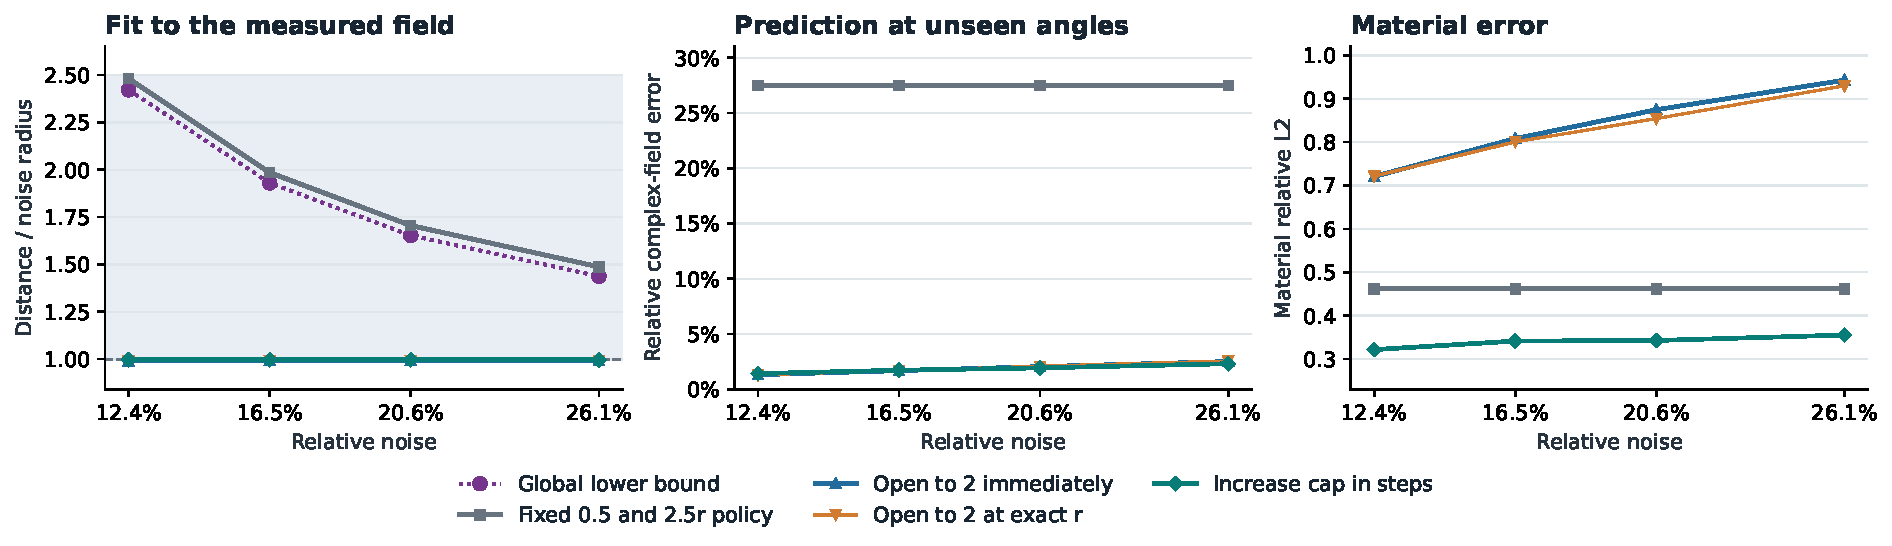
\includegraphics[width=\linewidth]{inversion-tradeoffs.pdf}
\caption{One compact object under four error levels. The lenient residual rule accepts the low-cap shape although the lower bound for the entire cap lies above the error radius. Immediate broad release improves prediction at unseen angles and worsens the final material error. Incremental release limits the excess peak.}
\label{fig:inversion-tradeoff}
\end{figure}

On the same exposed compact object we also compared incremental cap release at \(0.5,0.6,0.75,1,1.25,2\), with the same warm-start rule, material grid and point discrepancy test. Using the class result skips the infeasible first cap. Both policies first enter the ball at 0.75 and produce bitwise identical maps, with material relative errors of \(0.322\)--\(0.355\), interior errors of \(0.170\)--\(0.175\) and held-out field errors of 1.42--2.32\%. Guidance reduces objective calls from 22 to 19. Charging the cold class test in table~\ref{tab:cost} erases that time saving on the compact grid. This example establishes a class decision and a possible reduction in search work with reusable setup. The tested continuation already obtains the same reconstruction quality.

\FloatBarrier
